\documentclass[11pt,superscriptaddress,floatfix,notitlepage]{revtex4-1}
\usepackage{graphicx,subfigure,amsmath,bbm}
\usepackage{dcolumn}% Align table columns on decimal point
\usepackage{bm}% bold math
\usepackage{lipsum}
\usepackage{nameref}
% folowing  must be in this order
\usepackage{varioref}
\usepackage{hyperref}
\usepackage{cleveref}
\renewcommand{\familydefault}{\sfdefault}
\usepackage[]{sfmath}     %Equations in Arial
\newcommand{\minus}{\scalebox{0.75}[1.0]{$-$}}
\usepackage{float}
\usepackage[export]{adjustbox}
\usepackage{subscript}
\usepackage{color}
\usepackage{titlesec,setspace}
\usepackage[normalem]{ulem}
\usepackage{helvet}

\usepackage{setspace}
%\onehalfspacing

\allowdisplaybreaks

\renewcommand{\figurename}{{\bf Supplementary Figure}}
\renewcommand{\thefigure}{{\bf \arabic{figure}}}%
\renewcommand{\theequation}{\arabic{equation}}%
\renewcommand*{\citenumfont}[1]{#1}
\renewcommand*{\bibnumfmt}[1]{[#1]}
\bibliographystyle{naturemag}

\usepackage[font=sf,justification=raggedright,format=plain]{caption}

\begin{document} 

\begin{center}
    \Large{\bf Supplemental Information}
\end{center}

\noindent\textbf{Supplementary Note 1: The single- and three-band Hubbard Models} --- 
The Hamiltonian of the three-band Hubbard model is  
\begin{equation}
\begin{split}
H&=(\varepsilon_d-\mu)\sum_{i,\sigma}n_{i,\sigma}^d+ (\varepsilon_p-\mu)\sum_{j,\sigma} n^{p_\alpha}_{j,\sigma} 
+ \sum_{\langle  i,j\rangle,\sigma}t^{\phantom\dagger}_{ij}(d^\dagger_{i\sigma}p^{\phantom\dagger}_{\alpha j\sigma}+p^\dagger_{\alpha  j\sigma}d^{\phantom\dagger}_{i\sigma})\\
&+\sum_{\langle j,j^\prime \rangle,\sigma} t^{\phantom\dagger}_{jj^\prime}(p^\dagger_{\alpha j\sigma}p^{\phantom\dagger}_{\alpha^\prime j^\prime\sigma}+p^\dagger_{\alpha^\prime j^\prime\sigma}p^{\phantom\dagger}_{\alpha j\sigma}) + U^{\phantom\dagger}_{dd} \sum_i n^d_{i\uparrow}n^d_{i\downarrow} + U^{\phantom\dagger}_{pp} \sum_{j} n^{p_\alpha}_{j\uparrow}n^p_{j\downarrow}. 
\label{threeband}
\end{split} 
\end{equation}
Here, $d^\dagger_{i,\sigma}$ ($d^{\phantom\dagger}_{i,\sigma}$) creates (annihilates) a spin $\sigma$ ($=\uparrow,\downarrow$) hole in the copper $d_{x^2-y^2}$ orbital at site $i$;  $p^\dagger_{\alpha j\sigma}$ ($p^{\phantom\dagger}_{\alpha j\sigma}$) creates (annihilates) a spin $\sigma$ hole in the oxygen $p_\alpha$ ($\alpha = x,y$) orbital at site $j$; for nearest neighbor, $j=i\pm \hat{x}/2 \hspace{0.05cm} (\text{or} \hspace{0.1cm} \hat{y}/2)$; $n^d_{i\sigma}=d^\dagger_{i\sigma}d^{\phantom\dagger}_{i\sigma}$ and 
$n^{p_\alpha}_{j\sigma}=p^\dagger_{\alpha j\sigma}p^{\phantom\dagger}_{\alpha j\sigma}$ are the number operators; $\epsilon_d$ and $\epsilon_p$ are the onsite energies of the Cu and O orbitals, respectively; $\mu$ is the chemical potential; $t_{ij}$ is the nearest neighbor Cu-O hopping integral; $t_{jj^\prime}$ is the nearest neighbor O-O hopping integral; and $U_{dd}$ and $U_{pp}$ are the on-site Hubbard repulsions on the Cu and O orbitals, respectively. The hopping integrals are parameterized~\cite{Kung} as $t_{ij} = P_{ij}t_{pd}$ and $t_{jj^\prime} =  Q_{jj^\prime} t_{pp}$, where $P_{ij}=1$ for $j=i+\hat{y}/2$ or $j=i-\hat{x}/2$, $P_{ij}=-1$ for $j=i-\hat{y}/2$ or $j=i+\hat{x}/2$  and $Q_{jj^\prime}=1$ for $j'=j-\hat{x}/2+\hat{y}/2$ or $j'=j+\hat{x}/2-\hat{y}/2$, $Q_{jj^\prime}=-1$ for $j'=j+\hat{x}/2+\hat{y}/2$ or $j'=j-\hat{x}/2-\hat{y}/2$. Throughout, we adopted (in units of eV): $t_{pd} = 1.13$, $t_{pp} = 0.49$, $U_{dd} = 8.5$, $U_{pp} = 0$, and $\Delta = \varepsilon_p -\varepsilon_d = 3.24$~\cite{Kung,Czyzyk,Johnston,Ohta}, unless otherwise stated. Since we use a hole language, half-filling is defined as hole density $n_h=1$ and $n_h>1$ corresponds to hole-doping and $n_h<1$ corresponds to electron-doping. A finite $U_{pp}$ only leads to small quantitative changes in the pair structure (see Supplementary Figure~4), but worsens the sign problem significantly \cite{Kung}. Therefore, we keep $U_{pp}=0$ for this study except for the results presented in Supplementary Figure 4.

The downfolded single-band Hubbard model is 
\begin{equation}\label{singleband}
    H = -\mu\sum_{i \sigma} n_{i  \sigma} - \sum_{\langle  i,j\rangle \sigma} 
    t^{\phantom\dagger}_{ij}c^\dagger_{i \sigma}c^{\phantom\dagger}_{j \sigma} + 
    U \sum_{i}\left(n_{i \uparrow}-\frac{1}{2}\right)\left(n_{i \downarrow}-\frac{1}{2}\right),
\end{equation}
where $c^\dagger_{i \sigma}$ ($c^{\phantom\dagger}_{i \sigma}$) creates (annihilates) an electron with spin $\sigma$ at site $i$, $t_{i,j} = t$ and $t^\prime$ for nearest- and next-nearest-neighbor hoping, respectively, and zero otherwise. $U$ is the on-site Hubbard repulsion, and  $\mu$ is the chemical potential, which is adjusted to fix the electron filling. Throughout, we set $t = 1$, $U = 6t$, and vary $t^\prime$ as indicated in the text. 
\newline

\newpage\noindent\textbf{Supplementary Note 2: Symmetrized eigenvectors of the Bethe-Salpeter equation} --- To determine the structure of the effective pairing interaction, we solve the Bethe-Salpeter equation in the particle-particle singlet channel
\begin{equation} \label{eq:BSE}
    -\frac{T}{N_c} \sum_{K,\alpha_1,\dots,\alpha_4} \Gamma^{c, pp}_{\alpha,\beta,\alpha_1,\alpha_2}(K,K^\prime)\bar{\chi}^{\phantom\dagger}_{\alpha_1,\alpha_2,\alpha_3,\alpha_4}(K^\prime)  \phi^{R,\nu}_{\alpha_3\alpha_4}(K^\prime) = \lambda^{\phantom\dagger}_\nu \phi^{R,\nu}_{\alpha\beta}(K)\,.
\end{equation}
Here, $K=({\bf K},\text{i}\omega_n)$, and $\bar{\chi}_{\alpha_1,\alpha_2,\alpha_3,\alpha_4}({\bf K}, \text{i}\omega_n) = (N_c/N) \sum_{{\bf k}^\prime} [G_{\alpha_1\alpha_3}({\bf K+k'},\text{i}\omega_n)G_{\alpha_2\alpha_4}(-{\bf K}-{\bf k}^\prime, -\text{i}\omega_n)]$ is the coarse-gained bare particle-particle propagator. The irreducible particle-particle vertex $\Gamma^{c, pp}$ is extracted from the two-particle cluster Green's function $G^{2,c}_{\alpha_1,\alpha_2,\alpha_3,\alpha_4}(K,K')$ with zero center of mass momentum and frequency by inverting the cluster Bethe-Salpeter equation
\begin{equation}
\begin{split}
G^{2,c}_{\alpha_1,\alpha_2,\alpha_3,\alpha_4}(K,K^\prime)&=\bar{G}_{\alpha_1,\alpha_3}(K)\bar{G}_{\alpha_2\alpha_4}(-K)\delta_{K,K^\prime}
\\&\
+\frac{T}{N_c}\sum_{K^{\prime\prime},\alpha^\prime_1,\dots,\alpha^\prime_4}\bar{G}_{\alpha_1,\alpha^\prime_1}(K)\bar{G}_{\alpha_2,\alpha^\prime_2}(-K)\Gamma^{c,pp}_{\alpha^\prime_1,\alpha^\prime_2,\alpha^\prime_3,\alpha^\prime_4}(K,K^{\prime\prime})G^{2,c}_{\alpha^\prime_3,\alpha^\prime_4,\alpha_3,\alpha_4}(K^{\prime\prime},K^\prime)\,.
\label{BSE1}
\end{split}
\end{equation}
To remove the ambiguity between left and right eigenvectors of the eigenvalue equation (\ref{eq:BSE}), we symmetrize the pairing kernel entering Eq.~(\ref{eq:BSE}). Using matrix notation in $(K, \alpha, \beta)$, we first diagonalize the bare particle-particle propagator, $\bar{\chi}^D = U^{-1}\bar{\chi}U$, where $\chi^D$ is a diagonal matrix, to introduce the symmetrized BSE
\begin{equation}\label{sBSE}
-\frac{T}{N_c} U \sqrt{\chi^D}U^{-1} \Gamma^{c,pp} U \sqrt{\chi^D}U^{-1} \phi^\nu = \lambda_\nu \phi^\nu\,.
\end{equation}
We use the eigenvectors of the symmetrized BSE, $\phi^\nu_{\alpha\beta}(K)$, for the analysis presented in the main text. They are related to the right eigenvectors of the BSE in Eq.~(\ref{eq:BSE}) by 
\begin{equation}
    \phi^\nu = U\sqrt{\chi^D}U^{-1}\phi^{R,\nu}\,.
\end{equation}



\newpage\noindent\textbf{Supplementary Note 3: The basis transformation to the molecular $L$, $L^\prime$ orbitals} --- The construction of the Zhang-Rice singlet relies on a transformation from the oxygen $p_x$, $p_y$ orbital basis to bonding and anti-bonding molecular orbitals, denoted here 
as $L$ and $L^\prime$, respectively. The two basis are related by a unitary transformation \cite{ZhangRice,Avella2013,Maier4} defined in $k$-space  
\begin{equation}
L_{{\bf k}\sigma}=\frac{\text{i}}{\gamma_{{\bf k}}}~\left[\sin\left(\tfrac{k_xa}{2}\right)~p_{x{\bf k}\sigma}- \sin\left(\tfrac{k_ya}{2}\right)~p_{y{\bf k}\sigma}\right],\label{Lk}
\end{equation}
and
\begin{equation}
L^\prime_{{\bf k}\sigma}=-\frac{\text{i}}{\gamma_{{\bf k}}}~\left[\sin\left(\tfrac{k_ya}{2}\right)~p_{x{\bf k}\sigma}+ \sin\left(\tfrac{k_xa}{2}\right)~p_{y{\bf k}\sigma}\right],\label{Lbark}
\end{equation}
where $\gamma^2_{{\bf k}}=\sin^2(k_xa/2)+\sin^2(k_ya/2)$,  $p_{\alpha{\bf k}\sigma}=N^{-1/2}_c\sum_{j} p_{\alpha j \sigma}\exp(-\text{i}{\bf k} \cdot {\bf R}_j)$, and we have set the lattice constant $a = 1$. In this basis, only the $L$ state hybridizes with the Cu-$d$ orbital, while the $L^\prime$ state only hybridizes with the $L$ state. The Fourier transform of the $L$ and $L^\prime$ orbitals to real-space is defined as $L_{i\sigma}=N^{-1/2} \sum_{\bf k}L_{{\bf k}\sigma} \exp(-\text{i}{\bf k} \cdot {\bf R}_i)$, $L^\prime_{i^\prime\sigma}=N^{-1/2} \sum_{\bf k}L^\prime_{{\bf k}\sigma} \exp(-\text{i}{\bf k} \cdot {\bf R}_{i^\prime})$ where $i^\prime=i+\hat{x}/2+\hat{y}/2$.
\newline

\newpage\noindent\textbf{Supplementary Note 4: Superconducting transition temperature in the three-band Hubbard model} --- 
For the $6\times 6$ and $4\times 4$ DCA calculations presented in the main text, the QMC Fermion sign problem prevents calculations down to temperatures low enough to determine the superconducting transition temperature $T_c$ from the temperature where the leading eigenvalue of the Bethe-Salpeter equation crosses 1, i.e. $\lambda_d(T=T_c)=1$. This temperature can be reached on a $2\times 2$ cluster, however, and $T_c(n_h)$ can be determined as a function of hole density $n_h$ in that case. Supplementary Figure~\ref{Fig:dcaTcvsn2by2Upp0SM} shows the DCA results for $T_c(n_h)$ obtained in a $2\times 2$ cluster for the same model parameters as used in the main text. Similar to the electron-hole asymmetry found in Fig.~1 {\bf c} for the leading eigenvalue $\lambda_d(n_h)$ of the particle-particle Bethe-Salpeter equation, as well as the asymmetry found in experiments, the $T_c$ versus $n_h$ phase diagram exhibits a higher maximum $T_c$ on the hole doped side than on the electron-doped side. Moreover, these results are similar to previous DCA $2\times 2$ cluster calculations for a similar two-band model \cite{Macridin}, although the critical hole doping where $T_c$ vanishes is reduced compared to those earlier calculations. This difference may originate in the difference in model parameters, in particular the neglect of the direct oxygen-oxygen hopping $t_{pp}$ in the earlier two-band model calculations. 

\begin{figure}[ht]
\centering
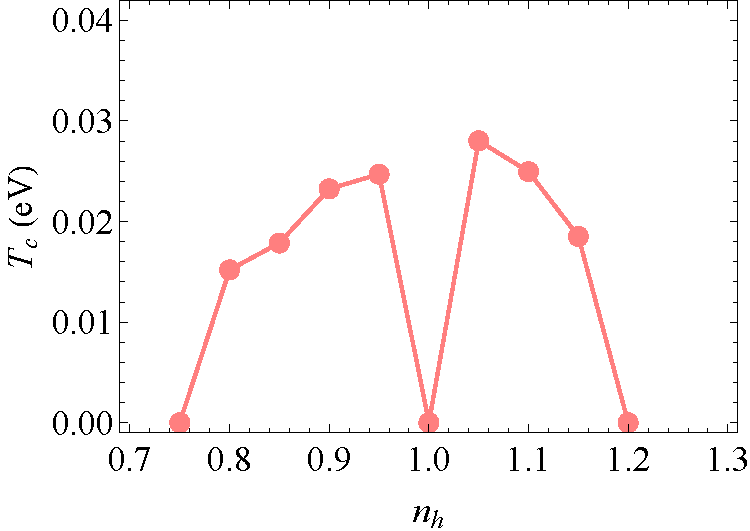
\includegraphics[width=0.5\linewidth]{./Figures/dcaTcvsn2by2Upp0SM.pdf}
\caption{{\bf Superconducting transition temperature as a function of filling for a $\mathbf{N_\text{Cu}\boldsymbol{=}2\boldsymbol{\times}2}$ DCA cluster}. The transition temperature $T_c$ is estimated by finding the temperature at which the leading BSE eigenvalue goes to $1$. The model parameters are (in units of eV) $\Delta = 3.24$, $t_{pd}=1.13$, $t_{pp}=0.49$, $U_{pp} = 0$, and $U_{dd}=8.5$. Our calculations find two superconducting domes on the hole-doped and electron-doped sides of the phase diagram, respectively, with a maximum $T_c$ that is higher for the hole-doped case, consistent  with experiments.}
\label{Fig:dcaTcvsn2by2Upp0SM}
\end{figure}


\newpage\noindent\textbf{Supplementary Note 5: Dependence of the leading eigenfunction on temperature, cluster size and oxygen Coulomb repulsion} --- 
While the leading eigenvalue $\lambda_d(T)$ shows a very strong increase with decreasing temperature, the temperature dependence of the corresponding eigenfunction is found to be rather weak. Supplementary Figure~2 shows how the orbital and spatial structure of the leading eigenfunction $\phi_{{\bf r}_\beta}({\bf r}_\alpha)$ of the (symmetrized) Bethe-Salpeter equation changes with decreasing temperature between $\beta=1/T=10$~eV$^{-1}$ (top panels {\bf a}-{\bf c} from Fig.~2 in the main text) and $\beta=12$~eV$^{-1}$ (bottom panels {\bf d}-{\bf f}). We only observe small quantitative changes between these two temperatures. 

\begin{figure}[h]
\centering
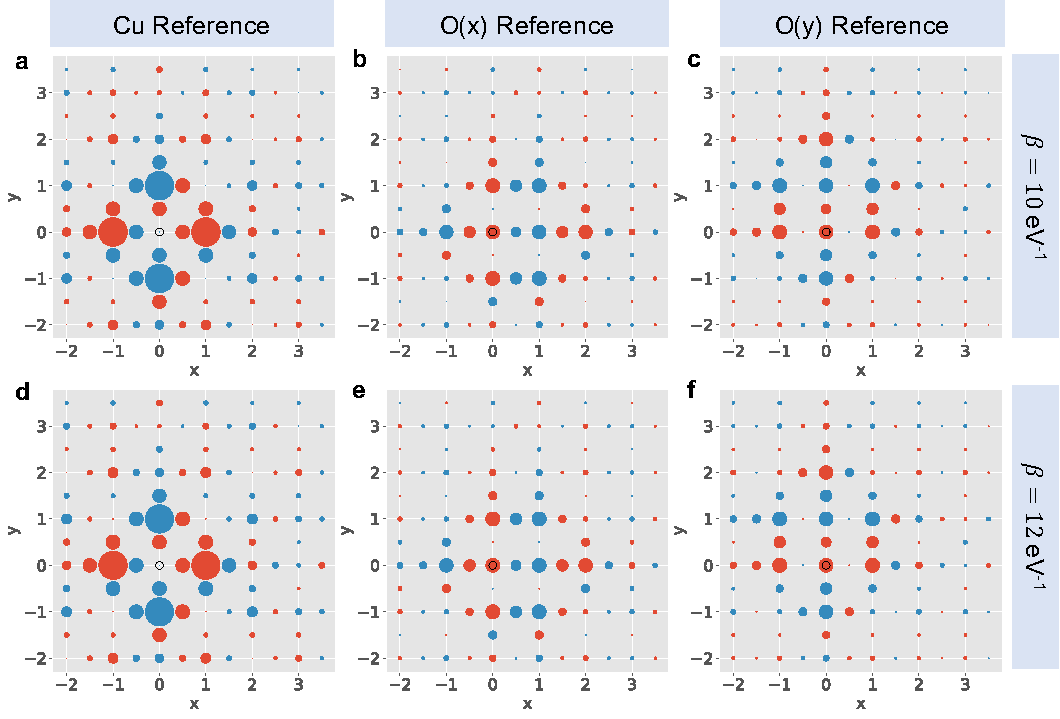
\includegraphics[width=\linewidth]{./Figures/DCAeigenvector6by6varyT.pdf}
\caption{{\bf Temperature dependence of the orbital structure of the pairs in the 
three-band model for the CuO\boldsymbol{$_2$} plane}. Each panel plots the real space components of the leading (symmetrized) eigenvector of the Bethe-Salpeter equation. The top and bottom rows show results obtained on a $N_\text{Cu}=6\times6$ cluster with a hole filling $n_h=1.15$ at an inverse temperature $\beta=10$ ~eV$^{-1}$ and $\beta=12$ ~eV$^{-1}$ respectively. The remaining model parameters are (in units of eV) $t_{pd}=1.13$, $t_{pp}=0.45$, $\Delta=3.24$, $U_{pp} = 0$, and $U_{dd}=8.5$. The left column describes the pairing between a Cu $d$ reference site and all other orbitals as a function of distance. The middle column describes pairings with respective to a p$_x$ orbital reference. The right column describes pairings with respective to a p$_y$ orbital orbital reference. All panels set the Cu $3d$ orbital at the origin, as labeled by the open ring. Only slight changes are observed in the pair structure between these two temperatures.}
\label{Fig:DCAeigenvector6by6varyT}
\end{figure}

The cluster size dependence of the leading eigenfunction is studied in Supplementary Figure~3, which shows the results of an $N_\text{Cu} = 4\times 4$ cluster calculation for a 15\% hole doped and a 15\% electron doped system. These results should be compared with Supplementary Figure~2 (or Fig.~2 in the main text), which displays the same calculation for a larger $N_\text{Cu}=6\times 6$ cluster. From this comparison, one sees that the $4\times 4$ cluster is large enough to contain the important components of the eigenfunction. Since the Fermion sign problem is much less severe in the $4\times 4$ cluster, it allows for calculations at lower temperatures or with an additional on-site Coulomb repulsion $U_{pp}$ on the oxygen orbitals. 

\begin{figure}[h]
\centering
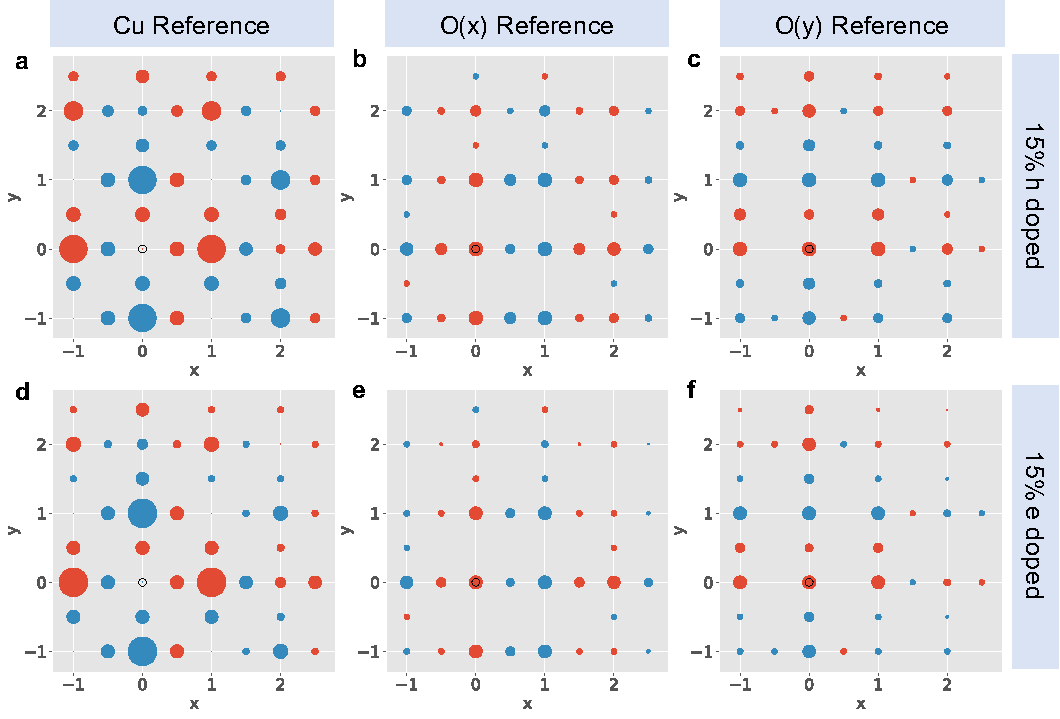
\includegraphics[width=\linewidth]{./Figures/DCAeigenvector4by4.pdf}
\caption{\textbf{The orbital structure of the pairs in the 
three-orbital model for the CuO\boldsymbol{$_2$} plane.} Each panel plots the real space components of the leading (symmetrized) eigenvector of the Bethe-Salpeter equation.  The top and bottom rows show results for hole- ($n_h=1.15$) and electron-doping ($n_h=0.85$), respectively, obtained on $N_\text{Cu} = 4\times 4$ clusters and at an inverse temperature $\beta=16$ ~eV$^{-1}$. The remaining model parameters are (in units of eV) $t_{pd}=1.13$, $t_{pp}=0.45$, $\Delta=3.24$, $U_{pp} = 0$, and $U_{dd}=8.5$. The left column describes the pairing between a Cu $d$ reference site and all other orbitals as a function of distance. The middle column describes pairings with respect to a p$_x$ orbital reference. The right column describes pairings with respect to a p$_y$ orbital orbital reference. All panels set the Cu $3d$ orbital at the origin, as labeled by the open ring. Compared with Fig.~2 in the main text, the $4\times4$ cluster contains the same essential pair structure as the $6\times 6$ cluster and makes it possible to explore lower temperatures and stronger interactions.}
\label{Fig:DCAeigenvector4by4}
\end{figure}

An additional $U_{pp} = 4.1$~eV term is considered in the data for the pair structure shown in Supplementary Figure~4. Other model parameters are unchanged from those considered in Supplementary Figure~3. Comparing these images with those in Supplementary Figure~3, one sees that the structure of the eigenfunction remains almost unchanged by the additional $U_{pp}$. Only a very slight suppression of the components that involve the O-$p$ orbitals is observed. This justifies the neglect of $U_{pp}$ in most of our calculations, and provides evidence that our main conclusions reached from those calculations are general and not affected by $U_{pp}$. 
\newline

\begin{figure}[h]
\centering
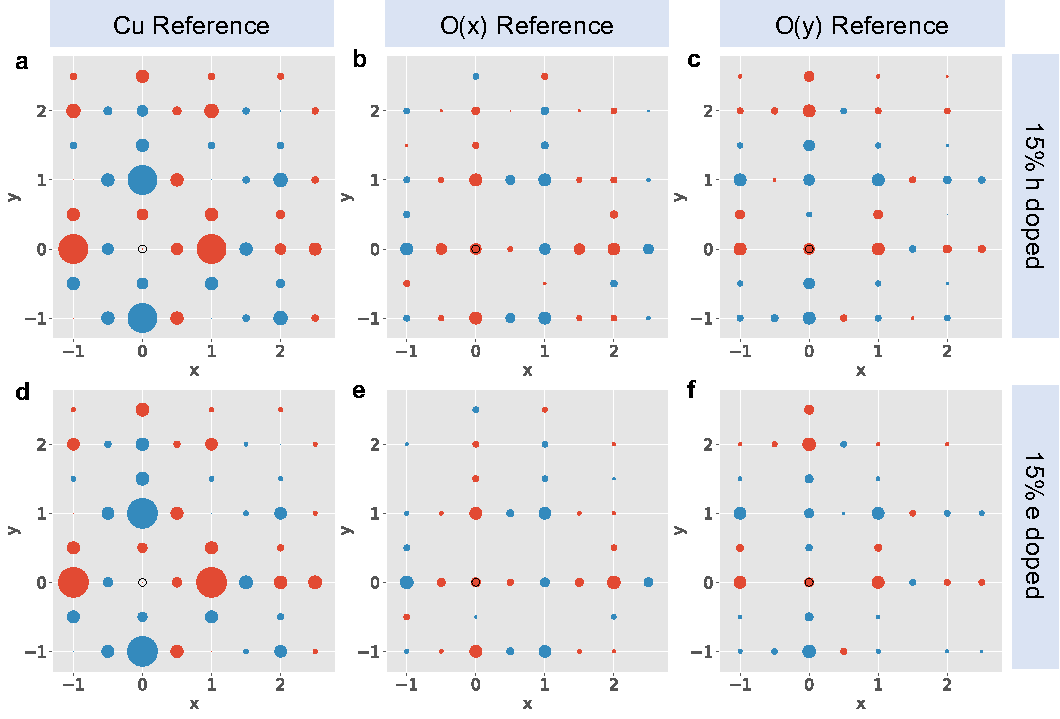
\includegraphics[width=\linewidth]{./Figures/DCAeigenvector4by4Upp41.pdf}
\caption{\textbf{Effect of finite $\mathbf{U_{pp}}$ on the orbital structure of the pairs in the three-band model with finite oxygen Coulomb repulsion $\mathbf{U_{pp}}$.} Each panel plots the real space components of the leading (symmetrized) eigenvector of the Bethe-Salpeter equation. The first and second rows show results for hole- ($n_h=1.15$) and electron-doping ($n_h=0.85$), respectively, obtained on $N_\text{Cu} = 4\times 4$ clusters and at an inverse temperature of $\beta=10$ ~eV$^{-1}$ and finite $U_{pp}=4.1$. The remaining model parameters are (in units of eV) $t_{pd}=1.13$, $t_{pp}=0.45$, $\Delta=3.24$ and $U_{dd}=8.5$. Compared to Supplementary Figure~\ref{Fig:DCAeigenvector4by4}, the effect of a finite $U_{pp}$ is very weak, with only a very slight suppression of the components that involve the O-$p$ orbitals. }
\label{Fig:DCAeigenvector4by4Upp41}
\end{figure}

\noindent\textbf{Supplementary Note 6: Role of the anti-bonding molecular $\mathbf{L^\prime}$ orbital} --- 
Finally, we show the components of the leading eigenfunction that involve the antibonding $L^\prime$ orbital in the bottom row of Supplementary Figure~5, compared to the bonding $L$ components that were already shown in Fig.~3 of the main text. From the results for the orbital hole densities in Fig.~4{\bf a} of the main text, it is clear that the $L^\prime$ molecular orbital remains almost completely unoccupied over the entire doping range considered, despite the finite hybridization between the $L$ and $L^\prime$ states. As a consequence, and as seen from the bottom row of Supplementary Figure~5, the $L^\prime$ state is not involved in the pairing. This provides strong support for the Zhang-Rice picture, which only considers the $d$- and $L$-states in the mapping to an effective single-band model. 

\begin{figure}[ht]
\centering
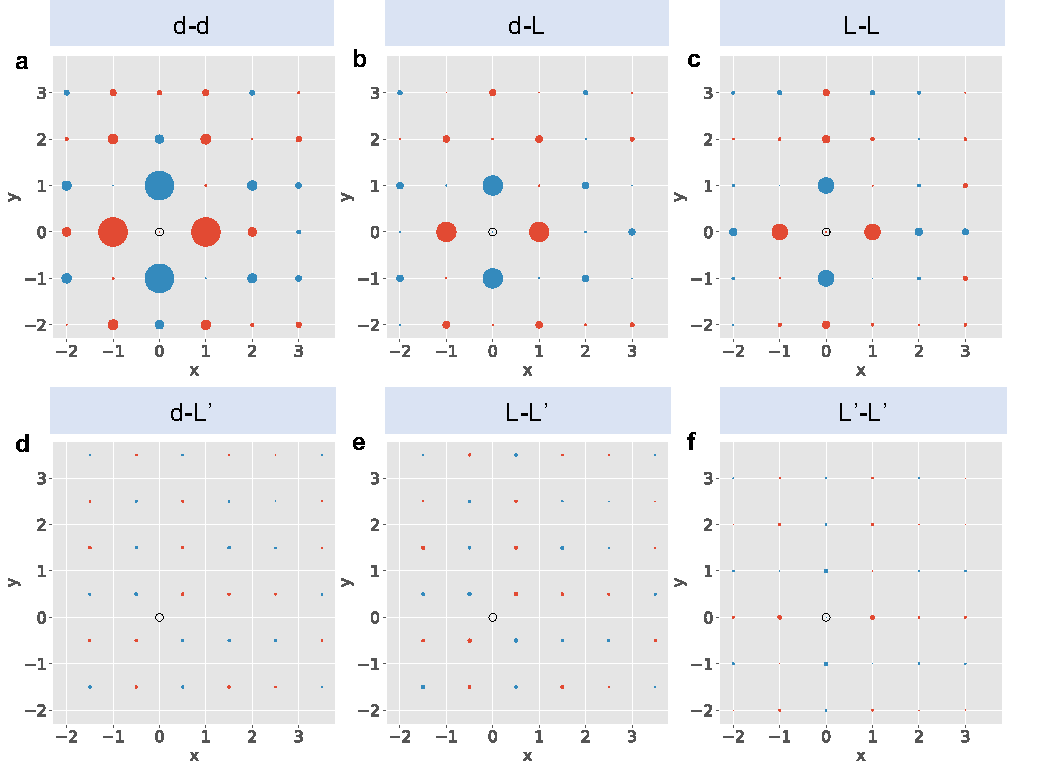
\includegraphics[width=\linewidth]{./Figures/Lbar.pdf}
\caption{\textbf{The $\mathbf{L^\prime}$-related components of the Cooper pairs in the three-band model for the CuO\boldsymbol{$_2$} plane.} $d$-$L^\prime$, $L$-$L^\prime$, $L^\prime$-$L^\prime$ pairing components are presented in panel {\bf d}, {\bf e}, {\bf f}, respectively, as compared with Panel {\bf a}-{\bf c} from Fig.~3 in the main text. All results were obtained  on a $N_\text{Cu} = 6\times6$ cluster with a filling $n_h=1.15$ and at an inverse temperature $\beta=10$ ~eV$^{-1}$. The remaining model parameters are (in units of eV) $t_{pd}=1.13$, $t_{pp}=0.49$, $U_{pp} = 0$, and $U_{dd}=8.5$. The same scale is used for the size of the points in the top and bottom rows. The pairing with the $L^\prime$-orbital is negligible.}
\label{Fig:weightvsdelta}
\end{figure}

\begin{thebibliography}{99}

\bibitem{Kung} Kung, Y.~F. \textit{et al.} Characterizing the three-orbital Hubbard model with determinant quantum Monte Carlo. \textit{Phys. Rev. B} {\bf 93}, 155166 (2016).

\bibitem{Czyzyk} Czy\.{z}yk M. T. \&  Sawatzky, G. A. Local-density functional and on-site correlations: The electronic structure of La$_2$CuO$_4$ and LaCuO$_3$. \textit{Phys. Rev. B} 49, 14211 (1994).

\bibitem{Johnston} Johnston, S.,  Vernay, F. \&  Devereaux, T. Impact of an oxygen dopant in Bi$_2$Sr$_2$CaCu$_2$O$_8$. \textit{Eur. phys. Lett.} {\bf 86}, 37007 (2009).

\bibitem{Ohta} Ohta, Y., Tohyama, T. \& Maekawa, S. Apex oxygen and critical temperature in copper oxide superconductors: Universal correlation with the stability of local singlets. \textit{ Phys. Rev. B} {\bf 43}, 2968 (1991).

\bibitem{ZhangRice}
Zhang, F. C. \& Rice, T. M. Effective Hamiltonian for the superconducting Cu oxides. \textit{Phys. Rev. B}  {\bf 37}, 3759(R) (1988).

\bibitem{Maier4} Z{\"o}lfl, M.~B., Maier, T.~A., Pruschke, T. \&  Keller, J. Electronic properties of CuO$_2$-planes: A DMFT study.
 \textit{Eur. Phys. J. B} {\bf 13}, 47 (2000). 

\bibitem{Avella2013} Avella, A., Mancini, F., Mancini, F. P. \& Plekhanov, E. Emery vs. Hubbard model for cuprate superconductors: a composite operator method study. \textit{Eur. Phys. J. B} {\bf 86}, 265 (2013). 

\bibitem{Macridin} Macridin, A., Jarrell, M., Maier, T.~A. \& Sawatzky, G.~A. Physics of cuprates with the two-band Hubbard model: The validity of the one-band Hubbard model. \textit{Phys. Rev. B} {\bf 71}, 134527 (2005).

\end{thebibliography}
\end{document}
